%
% teil1.tex -- Beispiel-File für das Paper
%
% (c) 2020 Prof Dr Andreas Müller, Hochschule Rapperswil
%
% !TEX root = ../../buch.tex
% !TEX encoding = UTF-8
%c
\section{Strömungsgleichungen\label{ueberschall:stroemungsgleichung}}
\kopfrechts{Strömungsgleichungen}
Wir untersuchen hier an einem einfachen Beispiel, 
illustriert in Abbildung~\ref{fig:wellblech},
die Strömung der Luft über einem Wellblech.
Dafür definieren wir das Potential als
\begin{align*}
    \Phi
    =
    U x + A \frac{l}{2 \pi} \sin\left(\frac{2 \pi x}{l}\right)
    e^{-\frac{2 \pi y}{l}}
\end{align*}
wobei $U$ die ungestörte Geschwindigkeit im 
Unendlichen $y\rightarrow\infty$ bedeutet.
% \documentclass{article}
% \usepackage{tikz}
% \usepackage{amsmath}

% \begin{document}
\begin{figure}
    \centering
    \resizebox{\textwidth}{!}{
    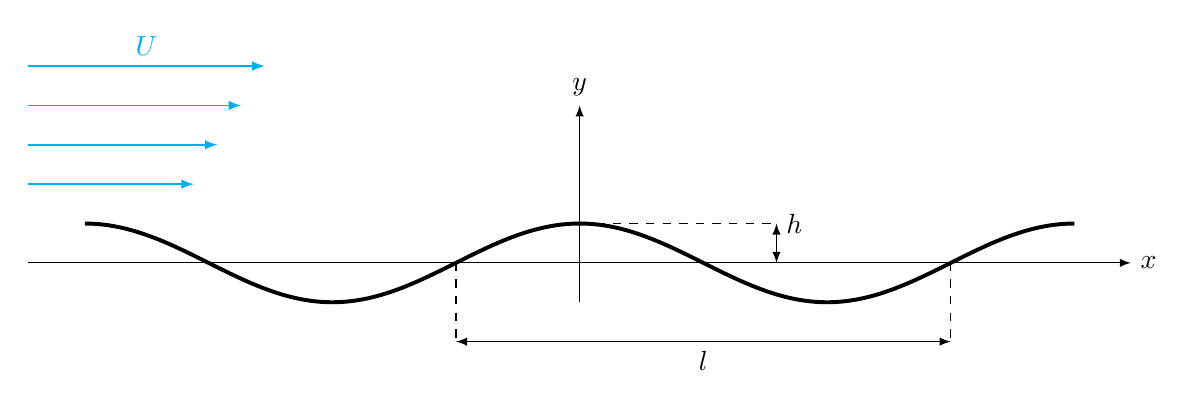
\begin{tikzpicture}[scale=1.0]
            % Achsen
        \def\startx{-7}
        \def\endx{-4}
        \def\starty{2.5}
        \def\ydis{0.5}
        \def\xenddis{0.3}
        \draw[->,>=latex] (-7, 0) -- (7, 0) node[right] {$x$};
        \draw[->,>=latex] (0, -0.5) -- (0, 2) node[above] {$y$};
        \draw[->,>=latex,cyan, line width=0.02cm] (\startx, \starty) -- (\endx, \starty) node[midway, yshift=0.25cm] {$U$};
        \draw[->,>=latex,cyan, line width=0.02cm] (\startx, \starty-\ydis) -- (\endx-\xenddis, \starty-\ydis);
        \draw[->,>=latex,cyan, line width=0.02cm] (\startx, \starty-2*\ydis) -- (\endx-2*\xenddis, \starty-2*\ydis);
        \draw[->,>=latex,cyan, line width=0.02cm] (\startx, \starty-3*\ydis) -- (\endx-3*\xenddis, \starty-3*\ydis);

        % % Gitterlinien optional
        % \draw[very thin, gray!30] (0, -1.5) grid[xstep=1, ystep=0.5] (7, 1.5);

        % Sinusfunktion
        \draw[thick, line width=0.05cm, black, domain=-2*pi:2*pi, samples=200] 
        plot (\x, {0.5*cos(\x r)});

        % Vermassungslinie l
        \def\xpos{0}
        \def\ypos{-1}
        \def\startmeas{-pi/2}
        \def\endmeas{3*pi/2}
        \draw[<->,>=latex] (\startmeas,\ypos) -- (\endmeas,\ypos) node[midway, below] {$l$};

        % Hilfslinien
        \draw[dashed] (\startmeas,\xpos) -- (\startmeas,\ypos);
        \draw[dashed] (\endmeas,\xpos) -- (\endmeas,\ypos);
        
        % Vermassungslinie h
        \def\xpos{2.5}
        \def\ypos{0}
        \def\startmeas{0}
        \def\endmeas{0.5}
        \draw[<->,>=latex] (\xpos,\startmeas) -- (\xpos,\endmeas) node[right] {$h$};

        % Hilfslinien
        \draw[dashed] (\startmeas,\endmeas) -- (\xpos,\endmeas);
        \draw[dashed] (\startmeas,\ypos) -- (\xpos,\ypos);
    \end{tikzpicture}
    }
    \caption{Strömung über einem Wellblech.}
    ~\label{fig:wellblech}
\end{figure}

% \end{document}


\subsection{Inkompressible Strömung im Unterschall}
Bei inkompressibler Strömung ist die
Laplace-Gleichung~\eqref{eq:laplace} sofort erfüllt.
Das kann bewiesen werden, indem wir für das Potential
die zweiten Ableitungen
\begin{align*}
    \frac{\partial^2 \Phi}{\partial x^2}
    &= \frac{A 2 \pi}{l} \sin\left(\frac{2 \pi x}{l}\right)
    e^{-\frac{2 \pi y}{l}} \\
    \frac{\partial^2 \Phi}{\partial y^2}
    &= -\frac{A 2 \pi}{l} \sin\left(\frac{2 \pi x}{l}\right)
     e^{-\frac{2 \pi y}{l}}
\end{align*}
berechnen wobei ersichtlich ist, dass
\begin{align*}
    \frac{\partial^2 \Phi}{\partial x^2}
    =
    -\frac{\partial^2 \Phi}{\partial y^2}.
\end{align*}
Die Laplace-Gleichung $\Delta \Phi = 0$ ist somit erfüllt.

Es existiert dann auch eine sogenannte Stromfunktion
\begin{align*}
    \Psi
    =
    U y - A \frac{l}{2 \pi} \cos\left(\frac{2 \pi x}{l}\right)
     e^{-\frac{2 \pi y}{l}},
\end{align*}
welche die Bedingung
\begin{align*}
    u 
    &=
    \frac{\partial \Phi}{\partial x}
    =
    \frac{\partial \Psi}{\partial y}
    \\
    v
    &=
    \frac{\partial \Phi}{\partial y}
    =
    -\frac{\partial \Psi}{\partial x}
\end{align*}
erfüllt.
$u$ und $v$ sind die Geschwindigkeitskomponenten in $x$- und $y$-Richtung.
Auch die Stromfunktion ist eine Lösung der Laplace-Gleichung
\begin{align*}
    \frac{\partial^2 \Psi}{\partial x^2}
    +
    \frac{\partial^2 \Psi}{\partial y^2}
    =
    0.
\end{align*}

Wenn wir $\Psi = c$ setzen, dann erhalten wir die Gleichung
\begin{align}
    c = U y - A \frac{l}{2 \pi} 
    \cos\left(\frac{2 \pi x}{l}\right) 
    e^{-\frac{2 \pi y}{l}}\label{eq:stromlinie}
\end{align}
einer Stromlinie.
Aufgelöst nach $y$ ergibt das
\begin{align*}
    y
    =
    \frac{A}{U} \frac{l}{2 \pi} 
    \cos\left(\frac{2 \pi x}{l}\right) 
    e^{-\frac{2 \pi y}{l}}.
\end{align*}
Wir setzen zusätzlich 
\begin{align*}
    \frac{A}{U} \ll 1,
\end{align*}
damit näherungsweise
\begin{align*}
    y
    =
    h \cos\left(\frac{2 \pi x}{l}\right)
\end{align*}
gilt.
Die Stromlinie sehr nahe am Wellblech ist eine
Kosinunslinie bzw. sie entspricht gerade der Kontur
des Blechs, wie in Abbildung~\ref{fig:stromlinien} ersichtlich.
\begin{figure}
    \centering
    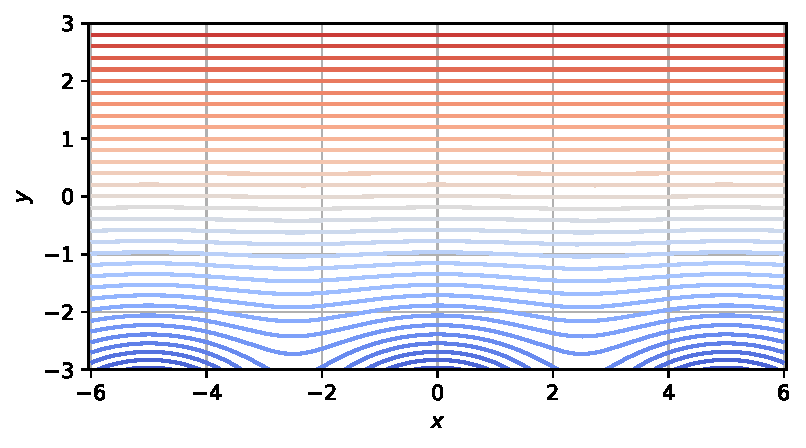
\includegraphics[width=\textwidth]{papers/ueberschall/figures/Stromlinien.pdf}
    \caption{Stromlinien über dem Wellblech für $\frac{A}{U}=0.2$.}
    ~\label{fig:stromlinien}  
\end{figure}
Die anderen Stromlinien $y > 0$ gehen mit zunehmendem $y$
in Gerade über, weil
\begin{align*}
    \lim_{y \to \infty}
    e^{-\frac{2 \pi y}{l}}
    =
    0.
\end{align*}

Mithilfe der bernoullischen Gleichung~\cite{BernoulliWikiDE}
\begin{align*}
    p_{\text{tot}} 
    = 
    p 
    + 
    \frac{1}{2} \rho V^2 
    + 
    \rho g z 
    = \text{const}
\end{align*}
lässt sich für dieses Szenario auch die Druckverteilung bestimmen.
Dabei ist $p_{\text{tot}}$ der Totaldruck, 
$\rho$ die Dichte des Fluids, $g$ die Erdbeschleunigung,
$V$ die Geschwindigkeit an einem Ort auf der Stromlinie 
und $z$ die Höhe über einem Bezugspunkt 
für ein dreidimensionales Strömungsfeld.
Da wir jedoch ausschliesslich in der $x,y$-Ebene arbeiten, 
fällt der letzte Term weg, weil $z = 0$.
Es bleibt somit:
\begin{align*}
    \underbrace{p}_{\text{statischer Druck}} 
    + 
    \underbrace{\frac{1}{2} \rho V^2}_{\text{dynamischer Druck}} 
    = 
    \text{const},
\end{align*}
was bedeutet, dass entlang einer Stromlinie 
der statische Druck und der dynamische Druck
zusammen konstant bleiben.
Wenn wir nun den lokalen Druck $p$ berechnen möchten, 
verwenden wir die freie Strömungsgeschwindigkeit $U$
als Referenzgrösse. 
Daraus ergibt sich:
\begin{align*}
    p_\infty 
    + 
    \frac{1}{2} \rho U^2 
    = 
    p 
    + 
    \frac{1}{2} \rho V^2,
\end{align*}
umgestellt nach dem lokalen Druck:
\begin{align*}
    p = p_\infty + \frac{1}{2} \rho (U^2 - V^2),
\end{align*}
wobei $V^2$ sich ergibt aus:
\begin{align*}
    V^2 = u^2 + v^2.
\end{align*}
Damit kann nun die Druckverteilung über dem Wellblech visualisiert werden, 
wie in Abbildung~\ref{fig:druckverteilung} dargestellt. 
Es handelt sich dabei um den relativen Druck, 
das heisst, der Druck ist bezogen auf den Umgebungsdruck. 
Deutlich erkennbar ist, dass der höchste Druck an den konkaven Stellen auftritt, 
während an den konvexen Stellen der niedrigste Druck herrscht.
\begin{figure}
    \centering
    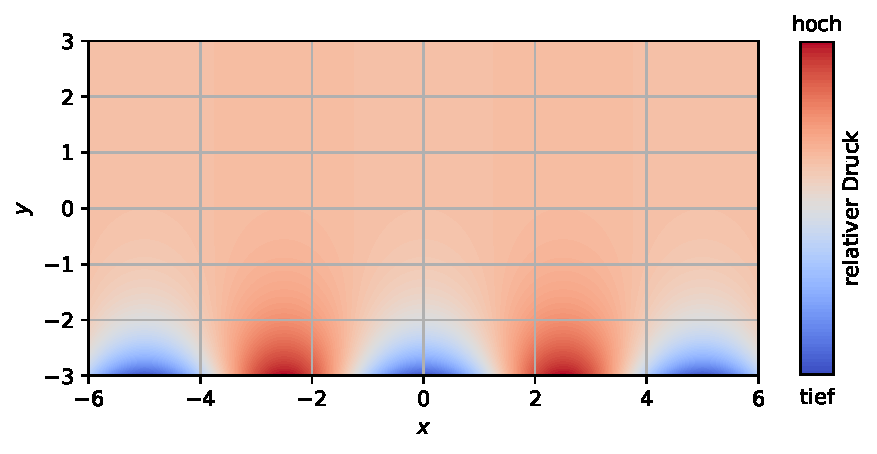
\includegraphics[width=\textwidth]{papers/ueberschall/figures/Druckverteilung.pdf}
    \caption{Relative Druckverteilung über dem Wellblech im Unterschall.}
    ~\label{fig:druckverteilung}  
\end{figure}

\subsection{Kompressible Strömung im Unterschall}
Bei kompressibler Strömung gestaltet sich die Situation etwas komplexer.
Die Ausgangslage ist eine partielle Differentialgleichung zweiter Ordnung,
die durch geeignete Vereinfachungen auf jene Terme reduziert wurde, 
welche den grössten Einfluss auf die Abweichung haben.
Das genaue Vorgehen ist in~\cite{Ackeret1928} ausführlich dokumentiert.
Die folgende Gleichung stellt daher eine Näherungslösung dar,
die jedoch wesentliche Eigenschaften der exakten Lösung widerspiegelt:
\begin{align}
    \frac{\partial^2 \Phi}{\partial x^2} 
    \left(1-\frac{U^2}{a^2}\right)
    +
    \frac{\partial^2 \Phi}{\partial y^2}
    =
    0.\label{eq:kompressible_stroemung}
\end{align}
Der Ausdruck in der Klammer ist eine Konstante, d.h.
durch die einfache Koordinatentransformation
\begin{align*}
    x 
    &=
    \xi \\
    y \beta
    &=
    \eta \\
    \beta
    &=
    \sqrt{1-\frac{U^2}{a^2}}
\end{align*}
wird daraus wenig überraschend die gewöhnlichen laplaceschen Gleichung
\begin{align*}
    \frac{\partial^2 \Phi}{\partial \xi^2} 
    +
    \frac{\partial^2 \Phi}{\partial \eta^2}
    =
    0,
\end{align*}
wie bei der Potentialströmung.
Das Potential dieser kompressiblen Strömung ergibt sich zu
\begin{align*}
    \Phi
    =
    U x + A \frac{l}{2 \pi} \sin\left(\frac{2 \pi x}{l}\right)
     e^{-\frac{2 \pi y \beta}{l}}
\end{align*}
und die dazugehörige Stromfunktion
\begin{align*}
    \Psi
    =
    U y - U \frac{h}{\beta^2} \cos\left(\frac{2\pi x}{l}\right)
     e^{-\frac{2\pi y \beta}{l}}.
\end{align*}
Durch gleiches Vorgehen wie bei Gleichung~\eqref{eq:stromlinie}
erhalten wir für $y \to 0$
\begin{align*}
    y
    =
    \frac{A \beta l}{2 \pi U} 
    \cos\left(\frac{2 \pi x}{l}\right).
\end{align*}
Damit wäre für kleine $y$ die Amplitude $h$ der Kosinuslinie
\begin{align*}
    h
    =
    \frac{A l \beta}{2 \pi U}
\end{align*}
und somit 
\begin{align*}
    A
    =
    \frac{2 \pi h U}{\beta l}.
\end{align*}
Demnach formulieren wir neu $\Phi$ als
\begin{align*}
    \Phi
    =
    U x + U \frac{h}{\beta} \sin\left(\frac{2 \pi x}{l}\right)
     e^{-\frac{2 \pi y \beta}{l}}.
\end{align*}
Der Faktor~$\beta$ beeinflusst das Abklingen der Störung,
wie in Abbildung~\ref{fig:abklingen_stromlinie} 
für drei verschiedene Fälle dargestellt ist.
Dazu werden die Stromlinien über einem Buckel visualisiert.
\begin{figure}
    \centering
    \begin{minipage}[b]{0.32\textwidth}
        \centering
        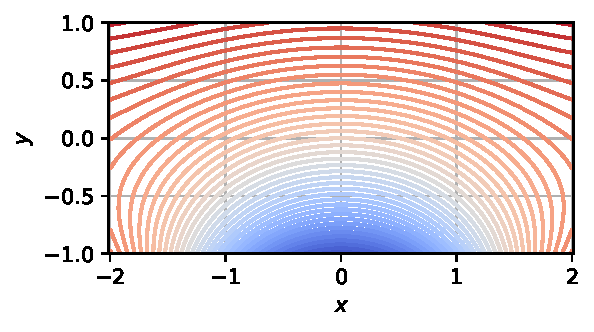
\includegraphics[width=\linewidth]{papers/ueberschall/figures/abklingen_10.pdf}
        \caption*{$\beta = 1$ ; $U = 10\,\frac{\mathrm{m}}{\mathrm{s}}$}
    \end{minipage}
    \hfill
    \begin{minipage}[b]{0.32\textwidth}
        \centering
        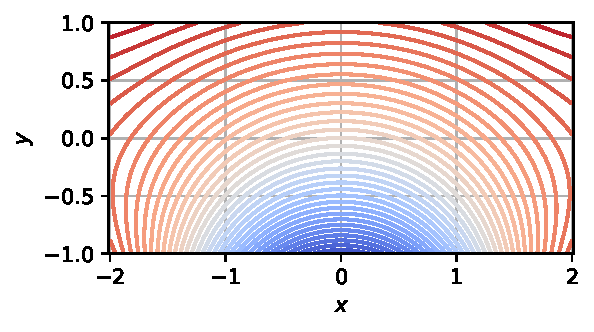
\includegraphics[width=\linewidth]{papers/ueberschall/figures/abklingen_200.pdf}
        \caption*{$\beta = 0.81$ ; $U = 200\,\frac{\mathrm{m}}{\mathrm{s}}$}
    \end{minipage}
    \hfill
    \begin{minipage}[b]{0.32\textwidth}
        \centering
        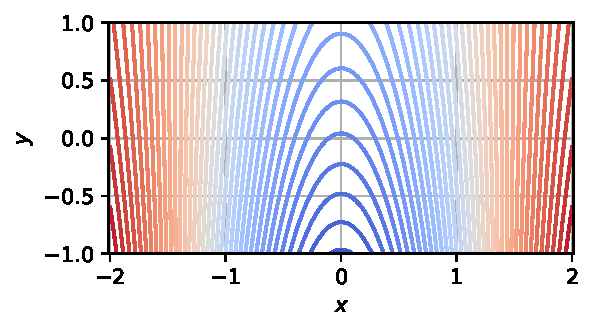
\includegraphics[width=\linewidth]{papers/ueberschall/figures/abklingen_340.pdf}
        \caption*{$\beta = 0$ ; $U = a$}
    \end{minipage}
    \caption{Stromlinien bei verschiedenen Strömungsgeschwindigkeiten im Unterschall.}
~\label{fig:abklingen_stromlinie}
\end{figure}

\subsection{Kompressible Strömung im Überschall}
Nun betrachten wir die Strömung im Überschallbereich.
Wir starten dabei bereits mit der vereinfachten 
Gleichung~\eqref{eq:kompressible_stroemung}:
\begin{align*}
    \frac{\partial^2 \Phi}{\partial x^2}
    \left(1 - \frac{U^2}{a^2}\right)
    =
    -\frac{\partial^2 \Phi}{\partial y^2},
\end{align*}
wobei der rechte Term zur besseren Übersicht auf die 
andere Seite genommen wurde.
Da im Überschallbereich $U > a$ gilt, wird der Ausdruck 
in der Klammer negativ.
Es ist daher sinnvoll, die Gleichung in der Form
\begin{align*}
    \frac{\partial^2 \Phi}{\partial x^2}
    \left(\frac{U^2}{a^2} - 1\right)
    =
    \frac{\partial^2 \Phi}{\partial y^2}
\end{align*}
umzuschreiben.
Führen wir nun eine geeignete Koordinatentransformation durch,
\begin{align*}
    x 
    &= 
    \xi, \\
    y \beta 
    &= 
    \eta,
\end{align*}
mit dem Parameter
\begin{align*}
    \beta = \sqrt{\frac{U^2}{a^2} - 1},
\end{align*}
so ergibt sich die transformierte Gleichung:
\begin{align}
    \frac{\partial^2 \Phi}{\partial \xi^2}
    -
    \frac{\partial^2 \Phi}{\partial \eta^2}
    =
    0.\label{eq:wellengl_ueberschall}
\end{align}
Diese Gleichung ähnelt formal der ursprünglichen Gleichung 
für den Unterschallbereich, weist jedoch ein 
unterschiedliches Vorzeichen im zweiten Term auf.
Dementsprechend handelt es sich hier um eine hyperbolische 
Differentialgleichung, die Wellenvorgänge beschreibt.
Das Strömungsverhalten im Überschallbereich ist daher — 
in gewisser Weise — mit dem Verhalten von Wellen in Wasser vergleichbar.

Die Lösung von Gleichung~\eqref{eq:wellengl_ueberschall} lautet:
\begin{align*}
    \Phi
    =
    F_1(\xi-\eta)
    +
    F_2(\xi+\eta).
\end{align*}
Für den vorliegenend Fall gilt sogar $F_2 = 0$, 
was zur Folge hat, dass für $\eta = \xi$ das Potential
$\Phi$ konstant ist.
So finden wir für $\Phi$
\begin{align*}
    \Phi
    =
    A \sin\left(
        \frac{2\pi}{l}
        (\eta-\xi)
    \right)
\end{align*}
und für $\Psi$
\begin{align*}
    \Psi
    =
    A \cos\left(
        \frac{2\pi}{l}
        (\eta-\xi)
    \right).
\end{align*}
In den Koordinaten $x$, $y$ entspricht $\eta = \xi$ gerade 
\begin{align*}
    y
    =
    \frac{x}{\sqrt{\frac{U^2}{a^2}-1}}.
\end{align*} 
Da aber der Anfangspunkt $x = 0$ und $y = 0$ beliebig gewählt
werden kann, ist $\Phi$ auf jeder unter dem Winkel
\begin{align*}
    \tan \alpha
    =
    \frac{1}{\sqrt{\frac{U^2}{a^2}-1}}.
\end{align*}
geneigten Geraden konstant.
Für $\sin \alpha$ ergibt sich
\begin{align*}
    \sin \alpha
    =
    \frac{\tan \alpha}{\sqrt{1 + \tan^2 \alpha}}
    =
    \frac{a}{U},
\end{align*}
$a$ ist auch bekannt als der mach-dopplersche Winkel.

Betrachten wir nun erneut die Druckverteilung, so erkennen wir in 
Abbildung~\ref{fig:druckvert_ueberschall} die sogenannten machschen Störungslinien. 
Diese sind besser bekannt als Schockwellen, 
die beim Durchbrechen der Schallmauer sichtbar werden. 
Auf jeder machschen Linie ist das Potential \(\Phi\) konstant. 
Alle Linien verlaufen parallel und besitzen die Steigung \(\tan \alpha\).
Ein exponentielles Abklingen, wie es im Unterschallfall auftritt, 
ist hier nicht mehr vorhanden. 
Die Maxima und Minima des Drucks entstehen nicht länger an den Wellenbergen, 
sondern befinden sich an den Wendepunkten der Wellenform. 
Dies liegt daran, dass an diesen Punkten die größte Neigung relativ zur 
ungestörten Anströmung mit Geschwindigkeit \(U\) vorliegt 
(siehe Abbildung~\ref{fig:wellblech}).
\begin{figure}
    \centering
    \begin{minipage}[b]{\textwidth}
        \centering
        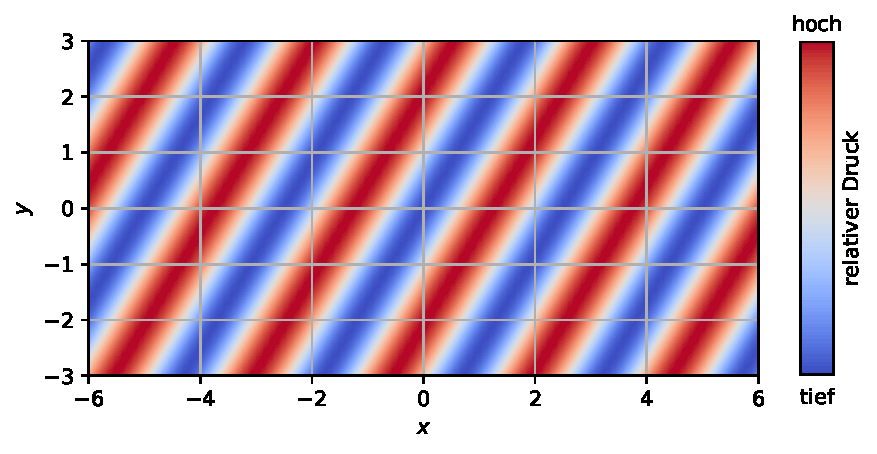
\includegraphics[width=\linewidth]{papers/ueberschall/figures/druck_mach_kegel_400.pdf}
        \caption*{$U = 400\,\frac{\mathrm{m}}{\mathrm{s}}$}
        ~\label{fig:druckvert_ueberschall_u400}
    \end{minipage}
    \hfill
    \begin{minipage}[b]{\textwidth}
        \centering
        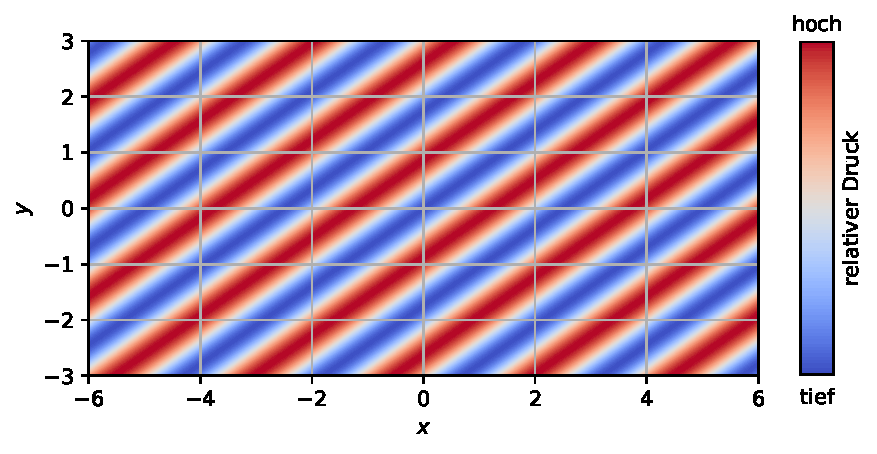
\includegraphics[width=\linewidth]{papers/ueberschall/figures/druck_mach_kegel_600.pdf}
        \caption*{$U = 600\,\frac{\mathrm{m}}{\mathrm{s}}$}
        ~\label{fig:druckvert_ueberschall_u600}
    \end{minipage}
    \caption{Relative Druckverteilung über dem Wellblech im Überschall.}
~\label{fig:druckvert_ueberschall}
\end{figure}